\chapter{\label{chapter:4_work-stealing}Case Of Study 1: Work-Stealing}

In this chapter, we will begin with a case of study related to the topic of relaxations applied to data structures. Our motivation for this study comes from previous research, which has shown that algorithms for concurrent objects often use expensive and complex synchronization mechanisms that can harm performance (see, for example~\cite{DBLP_conf_popl_AttiyaGHKMV11,DBLP_journals_toplas_Herlihy91}). To address this issue, researchers have proposed objects with relaxed semantics that can provide algorithms without the need for such costly mechanisms~\cite{maged.vechev.2009,fencefreework}. We aim to investigate whether there are any non-trivial and useful relaxed objects that can be implemented using only basic synchronization mechanisms without compromising performance. Specifically, we will be focusing on the case of work-stealing and exploring how we can provide relaxed data structures to solve this problem.

We will focus on First-In-First-Out (FIFO) data structures with single-producer multi-consumer semantics and in two relaxation methods for work-stealing, known as multiplicity~\cite{DBLP_journals_dc_CastanedaRR23} and weak-multiplicity. These relaxation methods allow a task to be extracted by more than one \Take/\Steal operation, but each process can only take the same task at most once. However, this relaxation can only occur in a concurrent environment. The first relaxation's property is directly guaranteed by the definition of set-linearizability. The second relaxation follows from the requirement that solutions must be sequentially exact. We will present two read/write, wait-free algorithms for these relaxations that do not require read-after-write synchronization patterns. Additionally, the second algorithm is fence-free with constant step complexity.

Chapter~\ref{chapter:6_Results} presents an experimental evaluation using three benchmarks related to this case study and the results obtained from the evaluation. Our goal is to determine whether implementation of the algorithms presented in this chapter can compete with or even surpass other state-of-the-art work-stealing algorithms. We implemented the algorithms using Java programming language.

\section{Introduction}

\emph{Work-stealing} is a popular technique to implement dynamic \emph{load balancing} for efficient task parallelization of irregular workloads. It has been used in several contexts, e.g., programming languages, parallel-programming frameworks, SAT solvers and state-space exploration in model checking (e.g.~\cite{DBLP_journals_tpds_AyguadeCDHLMTUZ09, DBLP_journals_jpdc_BlumofeJKLRZ96, CGSDKEPS05, DBLP_conf_jvm_FloodDSZ01, DBLP_conf_pldi_FrigoLR98, DBLP_conf_java_Lea00, DBLP_conf_hpca_RangerRPBK07}).

In work-stealing, each process \emph{owns} a set of tasks that must be executed. The \emph{owner} of the set can put tasks in it and can take tasks from it to execute them. When a process runs out of tasks (i.e., the set is empty), it becomes a \emph{thief} to steal tasks from a \emph{victim}. A work-stealing algorithm provides three high-level operations: \Put and \Take, which can be invoked only by the owner, and \Steal, which a thief can invoke. \emph{Linearizability} is the usual assumed correctness condition, while \emph{lock-freedom} and the stronger \emph{wait-freedom} are the typical  progress conditions.

A main target when designing work-stealing algorithms is to have \Put and \Take operations as simple and efficient as possible, as typically, they are the operations most intensively used by the owner. Unfortunately, it has been formally shown that any work-stealing algorithm in the standard asynchronous shared memory model must use \RAW synchronization patterns or atomic \RMW instructions (e.g., \CAS or \TAS)~\cite{DBLP_journals_jacm_AttiyaGHK09}. \RAW is a useful synchronization pattern based on the \emph{flag principle}, i.e., writing on a shared variable and then reading another variable (see~\cite {DBLP_books_daglib_0020056}). To correctly implement an algorithm using such a synchronization pattern in real multi-core architectures, a \emph{memory fence} needs to be explicitly added so that the compiler or the architecture does not reorder the \R and \W instructions. It is well-known that fences that avoid reads and writes to be reordered are highly costly, while atomic \RMW instructions, with high coordination power (which can be formally measured through the \emph{consensus number} formalism~\cite{DBLP_journals_toplas_Herlihy91}), are in principle slower than the simple \R/\W instructions.\footnote{In practice, contention might be the dominant factor, namely, an uncontended \RMW instruction can be faster than contended \R/\W instructions.} Indeed, the known work-stealing algorithms in the literature are based on the flag principle in their \Take/\Steal operations~\cite{circular.work.stealing, FLR98, non.blocking.work.stealing, 10.1145.571825.571876}.  Two possible ways to circumvent the impossibility result in~\cite{DBLP_journals_jacm_AttiyaGHK09} are to consider work-stealing with relaxed semantics or to make extra assumptions on the model. As far as we know,~\cite{maged.vechev.2009} and~\cite{fencefreework} are the only works that follow these directions.

Observing that in some contexts, it is ensured that no task is repeated (e.g., by checking first if a task is completed) or the nature of the problem solved tolerates repeatable work (e.g., parallel SAT solvers), Michael, Vechev, and Saraswat propose \emph{idempotent} work-stealing~\cite{maged.vechev.2009}, a relaxation allowing a task to be taken \emph{at least once}, instead of \emph{exactly once}. Three idempotent work-stealing algorithms are presented in~\cite{maged.vechev.2009}, where tasks are inserted/extracted in different orders. The relaxation allows each of the algorithms to circumvent the impossibility result in~\cite{DBLP_journals_jacm_AttiyaGHK09} in its \Put and \Take operations as they use only \R/\W instructions and are devoid of \RAW synchronization patterns. However, \Steal uses \CAS. Moreover, \Put requires that some \W instructions are not reordered, and \Steal requires that some \R instructions are not reordered either, and thus fences are required when the algorithms are implemented. However, fences between \R (resp. \W) instructions are usually not too costly. As for progress guarantees, \Put and \Take are wait-free while \Steal is only nonblocking.

Morrison and Afek consider the TSO model~\cite{DBLP_journals_cacm_SewellSONM10} and present two work-stealing algorithms in~\cite{fencefreework} whose \Put operation is wait-free and uses only \R/\W instructions,  and \Take and \Steal are either nonblocking and use \CAS, or blocking and use a \emph{lock}. The algorithms are non-trivial adaptations of the well-known Cilk THE and Chase-Lev work-stealing algorithms~\cite{circular.work.stealing, FLR98} to the TSO model. Generally speaking, in this model, \W (resp. \R) instructions cannot be reordered; hence, fences among \W (resp. \R) instructions are unnecessary. Additionally, each process has a local buffer where its \W instructions are stored until they are eventually propagated to the main memory (in FIFO order). Reordering some \W (resp. \R), instructions of Morrison and Afek's algorithms compromise correctness. However, TSO prevents this from happening. To avoid \RAW patterns, they assume bounded size \W buffers.

\section{\label{sec-ws-mult}Work-Stealing with Multiplicity}

Work-stealing with \emph{multiplicity} is a relaxation in which, roughly speaking, every task is extracted \emph{at least once}. If several operations extract the task, they must be \emph{concurrent}. In the formal set-sequential specification below (and its variant in the next section), tasks are inserted/extracted in FIFO order. The definition can be easily adapted to encompass other orders (e.g., LIFO). Figure~\ref{fig-example-execution} depicts an example of a set-sequential execution of work stealing with multiplicity, where concurrent \Take/\Steal operations extract the same task.

\begin{figure}[ht]
  \begin{center}
    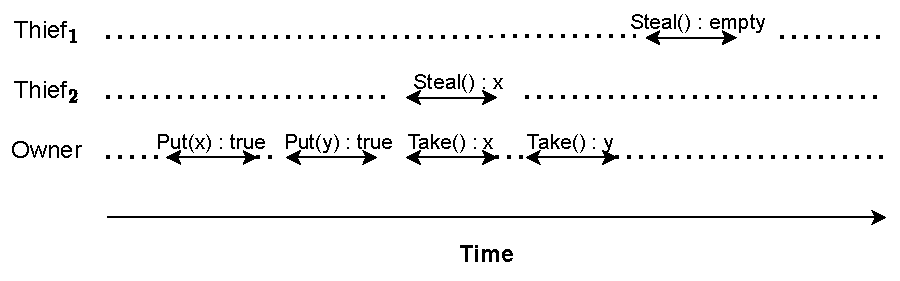
\includegraphics[width=0.6\textwidth]{contents/figures/IV_1_set-linearizability.pdf}
    \caption{\label{fig-example-execution}A set-sequential execution
      of work-stealing with multiplicity.}
  \end{center}
\end{figure}

\begin{definition}[FIFO Work-Stealing with Multiplicity\label{def-ws-mult}]

The universe of tasks that the owner can put is \(\mathbf{N} = \{ 1, 2, \hdots \}\), and the set of states \(Q\) is the infinite set of finite strings \(\mathbf{N}^*\).  The initial state is the empty string, denoted \(\epsilon\). In state \(q\), the first element in \(q\) represents the \emph{head} and the last one the \emph{tail}. The transitions are the following:

{\def\OldComma{,}
  \catcode`\,=13
  \def,{%
    \ifmmode%
    \OldComma\discretionary{}{}{}%
    \else%
    \OldComma%
    \fi%
  }%
  \begin{enumerate}

  \item \(\forall q \in Q\),
    \( \delta(q, \Put(x)) = (q \cdot x, \langle \Put(x): \true
    \rangle)\).

  \item \(\forall q \in Q, 0\leq t\leq n-1\), \(x \in \mathbf{N}\), \(
    \delta(x \cdot q, \{\Take(), \Steal_1(), \hdots, \Steal_t() \})
    = (q, \{ \langle \Take():x \rangle, \langle \Steal_1():x \rangle,
    \hdots, \langle \Steal_t():x \rangle \})\).

  \item \(\forall q \in Q\), \(1\leq t\leq n-1\), \(x \in \mathbf{N}\),
    \(\delta(x \cdot q, \{\Steal_1(), \hdots, \Steal_t() \}) =
    (q, \{\langle \Steal_1():x \rangle, \hdots, \langle
    \Steal_t():x \rangle\})\).

  \item \(\delta(\epsilon, \Take()) = (\epsilon, \langle \Take(): \epty
    \rangle)\).

  \item \(\delta(\epsilon, \Steal()) = (\epsilon, \langle \Steal(): \epty
    \rangle)\).

  \end{enumerate}}

\end{definition}

Let \(\mathcal A\) be a set-linearizable algorithm for work-stealing with multiplicity. Note that items 2 and 3 in Definition~\ref{def-ws-mult} and the definition of set-linearizability directly imply that in every execution of \(\mathcal A\), the number of \Take/\Steal operations that take the same task is, at most, the number of processes in the system, as the operations must be pairwise concurrent to be set-linearized together. Furthermore, every \emph{sequential} execution of \(\mathcal A\) (i.e., an execution where operations do not overlap in time) is a sequential execution of non-relaxed work-stealing, as every operation is linearized alone, by definition of set-linearizability. Formally, every sequential execution of \(\mathcal A\) is a sequential execution of (FIFO) work-stealing. We call this property \emph{sequentially-exact}.  Thus, without contention, \(\mathcal A\) provides an exact solution for (FIFO) work-stealing.

\begin{remark}~\label{remark-seq-exact-set-lin}
Every set-linearizable algorithm for work-stealing with multiplicity is sequentially-exact.
\end{remark}

\subsection{\label{sec-ws-mult-max-reg}Work-Stealing with Multiplicity from \MaxReg}


We show that work-stealing with multiplicity can be reduced to a single instance of a \MaxReg object (defined below). Together with any \R/\W wait-free linearizable algorithms for \MaxReg, our algorithm provides a \R/\W algorithm for work-stealing with multiplicity. We argue that using the \MaxReg algorithm of Aspnes, Attiya, and Censor-Hillel~\cite{DBLP_journals_jacm_AspnesAC12}, the resulting work-stealing algorithm with multiplicity has logarithmic step complexity, devoid of \RAW synchronization patterns. The algorithm presented in this section seems to have no practical implications. However, it will lead us to our efficient, fully fence-free \R/\W work-stealing algorithm with constant step complexity in all its operations.

Figure~\ref{figure-max-reg-mult} contains \WFWSM, a set-linearizable algorithm for work-stealing with multiplicity. The algorithm uses a linearizable wait-free \MaxReg object, which provides two operations: \MaxR, which returns the maximum value written so far in the object, and \MaxW, which writes a new value only if it is greater than the largest value written so far.


In \WFWSM, the tail of the queue is stored in the persistent local variable \(tail\) of the owner, while the head is stored in the shared \MaxReg \(Head\). Persistent means that the local variable retains its value between invocations to operations. When the owner wants to put a new task, it first locally increments \(tail\) (Line~\ref{A01}) and then stores the task in the corresponding entry of \(Tasks\) and marks one more entry with \(\bot\) (Line~\ref{A02}); \(\bot\) indicates lack of tasks. Recall that the notation in Line~\ref{A02} (instructions between brackets) denotes that the instructions can be executed in any order. When the owner wants to take a task, it first reads the current head of the queue from \(Head\) (Line~\ref{A04}). Then, if there are tasks available (i.e., the head is less or equal to the tail), it reads the task at the head, updates \(Head\), and finally returns the task (Lines~\ref{A06} and~\ref{A09}); if there are no tasks available, the owner returns $\epty$ (Lines~\ref{A11}). When a thief wants to steal a task, it first reads the current value of \(Head\) (Line~\ref{A12}) and then reads that entry of \(Tasks\) (Line~\ref{A13}). If it reads a task (i.e. a non-\(\bot\) value), it updates \(Head\) and then returns the task (Lines~\ref{A16} and~\ref{A17}).  Otherwise, all tasks have been extracted, and it returns \epty (Line~\ref{A19}).

The semantics of \MaxW guarantees that $Head$ contains the current value of the head at all times, as a ``slow'' process cannot ``move back'' the head by writing a smaller value in \(Head\) (in Lines~\ref{A06} or~\ref{A16}). Thus, the \MaxReg \(Head\) acts as a sort of barrier in the algorithm. Two \Take/\Steal operations can return the same task only if concurrent, reading the same value from \(Head\).

%==================================================================
\begin{figure}[H]
  \centering
  \fbox{
    \begin{minipage}[t]{150mm} \footnotesize
      \renewcommand{\baselinestretch}{2.5} \resetline
      \begin{tabbing} aaaa\=aa\=aa\=aa\=aa\=aa\=aa\=\kill %~\\

        {\bf Shared Variables:}\\
        \> \> \(Head\): atomic $\MaxReg$ object initialized to \(1\)\\
        \> \> \(Tasks[1, 2, \hdots]\): array of atomic $\R/\W$ objects
        with\\ \>\>\>\>\>\>\> the first two objects initialized to \(\bot\)\\

        {\bf Local Variables of the Owner:}\\
        \> \> \(tail \leftarrow 0\)\\ \\

        {\bf Operation} \(\Put(x)\): \\
        \line{A01} \> \> \(tail \leftarrow tail + 1\)\\
        \line{A02} \> \> \(\{Tasks[tail].\W(x),\ Tasks[tail + 2].\W(\bot)\}\)\\
        \line{A03} \> \> {\bf return } $\true$\\
        {\bf end} $\Put$ \\ \\

        {\bf Operation} \(\Take()\): \\
        \line{A04} \> \> \(head \leftarrow Head.\MaxR()\)\\
        \line{A05} \> \> {\bf if \(head \leq tail\) then}\\
        \line{A06} \> \> \> \(\{ x \leftarrow Tasks[head].\R(),
        Head.\MaxW(head+1)\}\)\\
        % \line{A07} \> \> $head \leftarrow head+1$\\
        % AC: Miguel ya habia observado que la sigueinte linea no es
        % necesaria. Yo no habia entendido
        % \line{A08} \> \> $Head.\MaxW(head)$\\
        \line{A09} \> \> \> {\bf return} \(x\)\\
        \line{A10} \> \> {\bf end if}\\
        \line{A11} \> \> {\bf return} $\epty$\\
        {\bf end} $\Take$ \\ \\


        {\bf Operation} \(\Steal()\): \\
        \line{A12} \> \> \(head \leftarrow Head.\MaxR()\)\\
        \line{A13} \> \> \(x \leftarrow Tasks[head].\R()\) \\
        \line{A14} \> \> {\bf if \(x \neq \bot\) then}\\
        % \line{A15}\>  \> \> $head \leftarrow head+1$\\
        \line{A16} \> \> \> \(Head.\MaxW(head+1)\)\\

        \line{A17} \> \> \> {\bf return} \(x\)\\
        \line{A18} \> \> {\bf end if}\\
        \line{A19} \> \> {\bf return} $\epty$\\
        {\bf end} $\Steal$

      \end{tabbing}
    \end{minipage}
  }
  \caption{\label{figure-max-reg-mult}\WFWSM: a \MaxReg-based
    set-linearizable algorithm for work-stealing with multiplicity.}
\end{figure}
% =================================================================

Note that if only the first object in \(Tasks\) is initialized to \(\bot\) (and hence \Put has modified accordingly), a thief may read a value from \(Tasks\) that has not been written by the owner: in execution with a single \(\Put(x)\) operation, the steps in Line~\ref{A02} could be executed \(Tasks[1].\W(x)\) first and then \(Tasks[2].\W(\bot)\) with a sequence of two \Steal operations completing in between, resulting in the second operation reading $Tasks[2]$, which has not been written yet by the owner, and might contain a value distinct from \(\bot\).


\begin{theorem}\label{theo-wf}
\WFWSM (Figure~\ref{figure-max-reg-mult}) is a set-linearizable wait-free algorithm for work-stealing with multiplicity, using \R/\W instructions and a single instance of a linearizable \MaxReg object. Moreover, all operations execute a constant number of \R/\W instructions, invoke a constant number of operations of the \MaxReg object, and \Put is \R/\W.
\end{theorem}

\begin{proofT}
The algorithm is wait-free since the \MaxReg object is assumed to be wait-free, and none of the operations executes a loop. Observe that \Put uses only \R/\W. Before proving that \WFWSM is set-linearizable, we first observe that at any time, the thieves read the range of \(Tasks\) that the owner has already initialized; more specifically, every \Steal operation reads from \(Tasks\) (in Line~\ref{A13}), a value that was written by the owner, either \(\bot\) or a task.

In any given execution, the range \(Tasks[Head, Head+1, \hdots, ]\) contains a (possibly empty) sequence of tasks followed by at least one \(\bot\) value, considering the entries in index-ascending order. The claim is true initially as the first two entries if \(Tasks\) are initialized to \(\bot\). Every time the owner stores a new task, it initializes a new entry of \(Task\) to \(\bot\) (Line~\ref{A02}); hence the claim holds at any time, as \(Head\) is incremented only if the owner or a thief reads that \(Tasks[Head]\) contains a non-\(\bot\) value (Lines~\ref{A06} or~\ref{A16}).  Note that the order of the instructions in Line~\ref{A02} is irrelevant.

We now prove that \WFWSM is set-linearizable. Consider any finite execution \(E\) of it. Since we already argued the algorithm is wait-free, there is a finite extension of \(E\) in which all its operations are completed, and no new operations start. Thus, we can assume that there are no pending operations in \(E\).

First, note that the semantics of \MaxW implies that no pair of non-concur-rent \Take/\Steal operations return the same task: if two operations are not concurrent, then the first one increments the value of \(Head\), the second operation cannot read the same tasks from \(Tasks\). Thus, we have:

\begin{remark}\label{remark-concurrency}
If a task is returned by more than one \Take/\Steal operation, these operations are pairwise concurrent. Thus, two distinct \Take operations cannot return the same task.
\end{remark}


The main observation for the set-linearizability proof is that, at any time, the state of the object is represented by the tasks in the range \(Tasks[Head, Head+1, \hdots ]\), i.e., the sequence of non-\(\bot\) values (in index-ascending order) written by the owner in that range. The set-linearization \(\SetLin(E)\) of \(E\) is obtained as follows:

\begin{itemize}

\item Every \Put operation is set-linearized \emph{alone} (i.e., in a concurrency class containing only that operation) placed at its step corresponding to \(Tasks[tail]\). \(\W(x)\) in \(E\) (Line~\ref{A02}).

\item For every task returned by at least one \Take/\Steal operation, all operations returning the task are set-linearized in the same concurrency class placed at the first step \(e\) of \(E\) that corresponds to \(Head.\MaxW(head+1)\) (either Line~\ref{A06} or~\ref{A16}) among the steps of the operations. Note that \(e\) occurs between the invocation and response of every operation in the concurrency class. Since the operations return the same task, all of them execute the \MaxR steps in Lines~\ref{A04} or~\ref{A12} before \(e\), and, by definition, \(e\) appears in \(E\) before any other operation executes its step corresponding to \(Head.\MaxW(head+1)\). Observe that the order in which the instructions in Line~\ref{A06} are executed is irrelevant.

\item Every \Take operation returning \epty is set-linearized alone, placed at its step in \(E\) corresponding to\\ \(Head.\MaxR()\) (Line~\ref{A04}).

\item Every \Steal operation returning \epty is set-linearized alone, placed at its step in \(E\) corresponding to \(Head.\MaxR()\) (Line~\ref{A12}).

\end{itemize}

Every concurrency class of \(\SetLin(E)\) is placed at a step of \(E\) that lies between the invocation and response of each operation in the concurrency class, which immediately implies that \(\SetLin(E)\) respects the partial order \(<_E\) of~\(E\). Thus, to conclude that \(\SetLin(E)\) is a set-linearization of \(E\), we need to show that it is indeed a set-sequential execution of work-stealing with multiplicity.

First, a task can be extracted by a \Take/\Steal operation only if the \Put operation that stores the task executes its step corresponding to \(Tasks[tail].\W(x)\) (in Line~\ref{A02}) before the \Take/\Steal operation reads the entry of \(Tasks\) where the task is stored. Thus, in \(\SetLin(E)\), every task is inserted before it is extracted.

Now, \Put stores tasks in \(Tasks\) in index-ascending order. Due to the semantics of \MaxReg, \(Head\) never ``moves back'', i.e., it only increases by one at a time, and hence \Take and \Steal extract tasks in index-ascending order too. Tasks in \(\SetLin(E)\) are inserted/extracted in FIFO order.

More specifically, for any concurrency class \(C\) of \(\SetLin(E)\) with \Take/\Steal operations that return the same task~\(x\), right before the step \(e\) of \(E\) where \(C\) is set-linearized, we have that \(x\) is a task with the smallest index (left-most) in the range \(Tasks[Head, Head+1, \hdots]\), and thus indeed the operations in \(C\) get the ``oldest" task in the object.

It only remains to be argued that any \Take/\Steal operation that returns \epty, does so correctly, i.e., each of these operations is set-linearized at a step of \(E\) at which \(Tasks[Head, Head+1, \hdots]\) is empty, i.e., all its entries initialized by the owner in that range contain \(\bot\).

Consider any \Take operation in \(E\) that returns \(\epty\).  Observe that this can happen only if the owner sees that \(head > tail\), namely, the conditional of Line~\ref{A05} is not satisfied. This is possible only when no task has been inserted, or all items have been extracted, and hence \(Tasks[Head, Head+1, \hdots]\) is empty. Consider any \Steal operation in \(E\) that returns \(\epty\).  This is possible only when the thief reads \(\bot\) from \(Tasks\) in Line~\ref{A13}, and since we already argued that the owner inserts tasks in ascending order, the sequence \(Tasks[Head, Head+1, \hdots]\) is empty.

We conclude that \(\SetLin(E)\) is a valid set-sequential execution of work-stealing with multiplicity, and as it respects the partial order \(<_E\) of \(E\), we have that it is a set-linearization of \(E\), and therefore \WFWSM is set-linearizable. The theorem follows.
\end{proofT}

If we replace \(Head\) with the \R/\W\ wait-free linearizable \MaxReg algorithm of Aspnes, Attiya, and Censor-Hillel~\cite{DBLP_journals_jacm_AspnesAC12}, whose step complexity is \(O(\log m)\), where \(m \ge 1\) is the maximum value that can be stored in the object, the step complexity of \WFWSM is bounded wait-free with logarithmic step complexity too. In the resulting algorithm, at most $m$ tasks can be inserted; the actual value of m is application-dependent. Since the algorithm does not use \RAW synchronization patterns (as explained in the proof of Theorem~\ref{theo-wf-log}), the resulting algorithm does not use those patterns either.

\begin{theorem}\label{theo-wf-log}
If $Head$ is an instance of the \R/\W\ wait-free linearizable \MaxReg algorithm of Aspness, Attiya, and Censor-Hillel~\cite{DBLP_journals_jacm_AspnesAC12}, \WFWSM is set-linearizable, fully \R/\W and \Take and \Steal have step complexity $O(\log m)$, where $m$ denotes the maximum number of tasks that can be inserted in an execution.  Furthermore, no operation uses \RAW synchronization patterns.
\end{theorem}

\begin{proofT}
The algorithm remains set-linearizable by the composability of set-linearizability \cite{DBLP_journals_jacm_CastanedaRR18}. While the step complexity of \Put is $O(1)$, the step complexity of \Take and \Steal is $O(\log m)$ as the step complexity \MaxR and \MaxW of the \MaxReg algorithm~\cite{DBLP_journals_jacm_AspnesAC12} is $O(\log m)$.

We now argue that \Take and \Steal do not use \RAW synchronization patterns. The reason is that the \MaxReg algorithm does not use this synchronization mechanism. Roughly speaking, the algorithm consists of a binary tree of height $O(\log m)$ with an atomic bit in each node.  When a process wants to perform \MaxR, it reads the bits in the path of the tree from the root to a leaf and then returns a value according to the leaf it reached; the next node in the path the process reads depends on the current node's value. When a process wants to perform \MaxW, it reads the bits in a path from the root to a leaf, which is a function of the binary representation of the value the process wants to write; then, if the new value is larger than the current one, in a bottom-up manner, it writes 1 in every node in the path with 0 (for the algorithm to be linearizable, the writes should occur in this order. Hence the algorithm is not fence-free). Thus, we have that \MaxR consists of a sequence of reads, and \MaxW consists of a sequence of reads followed by a (possibly empty) sequence of writes. Therefore, \Take/\Steal of \WFWSM consists of a sequence of reads followed by a (possibly empty) sequence of writes, and thus the operation does not use \RAW synchronization patterns.
\end{proofT}

\section{\label{sec-ws-nc-mult}Work-Stealing with Weak Multiplicity}

A logarithmic step complexity of the \Take{}~operation is prohibitive in practical settings. Ideally, we would like to have constant step complexity in all operations and use simple synchronization mechanisms if possible. In this section, we propose a variant of work-stealing with multiplicity that admits fully \R/\W fence-free algorithms with constant step complexity in all its operations. Intuitively, the variant requires that every task is extracted at least once, but now every process extracts a task \emph{at most once}, hence \Take/\Steal~operations returning the same task \emph{might not} be concurrent. Therefore, the relaxation retains the property that the number of operations that can extract the same task is, at most, the number of processes in the system. We call this relaxation \emph{weak multiplicity}.

\begin{figure}[H]
  \centering
  \subfloat[\label{fig-state-weak}A schematic view of work-stealing
  with weak multiplicity.] {
    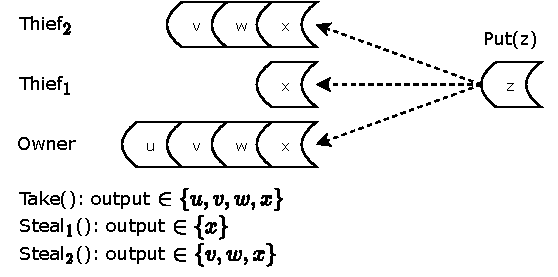
\includegraphics[width=0.45\textwidth]{contents/figures/IV_2_work_stealing}
  }
  \hfill
  \subfloat[\label{fig-example-execution-weak}A sequential execution
  of work-stealing with weak multiplicity.] {
    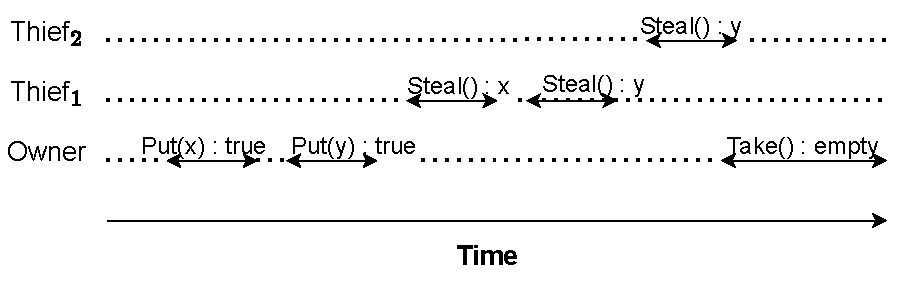
\includegraphics[width=0.45\textwidth]{contents/figures/IV_3_work_stealing_weak_multiplicity}
  }
  \caption{\label{fig-weak-mult} Schematic view and sequential
    execution of work-stealing with weak multiplicity.}
\end{figure}



Figure~\ref{fig-state-weak} depicts a schematic view of work stealing with weak multiplicity. Intuitively, each process has its own \emph{virtual} queue of tasks at any state. When the owner inserts a new task, it \emph{atomically} places the task in all virtual queues, as shown in the figure. Therefore, for any pair of processes' virtual queues, one is a suffix of the other. A \Take/\Steal operation can return any task from its virtual queue that is no ``beyond'' the first task of the \emph{shortest} virtual queue in the state. In the example depicted in the figure~\ref{fig-state-weak}, a \Steal operation of thief $p_1$, denoted $\Steal_1()$, can return only $x$, as $p_1$ has the shortest virtual queue in the state. In contrast, a \Take operation can return any task in its virtual queue and remove all preceding tasks. E.g., if $w$ is returned, then $u$ and $v$ are removed from the virtual queue, which leaves the owner's virtual queue containing only $x$ and $z$. Note that tasks are extracted in FIFO order. This property guarantees that every task is taken at least once. In our algorithms, \emph{all} virtual queues are implemented using a single queue. Figure~\ref{fig-example-execution-weak} shows an example of sequential execution of work-stealing with weak multiplicity. Note that \Take/\Steal operations can get the same task, although they are not concurrent.

The next \emph{sequential} specification formally defines work-stealing with weak multiplicity. Without loss of generality, the specification assumes that \(p_0\) is the owner and each invocation/response of thief \(p_i\) is subscripted with its index, which belongs to the set \(\{1, \hdots, n-1\}\).



\begin{definition}[FIFO Work-Stealing with Weak Multiplicity\label{def-ws-nc-mult}]
The universe of tasks that the owner can put is \(\mathbf{N} = \{ 1, 2, \hdots \}\), and the set of states \(Q\) is the infinite set of \(n\)-vectors of finite strings \(\mathbf{N}^* \times \hdots \times \mathbf{N}^*\), with the property that for any two pairs of strings in a vector/state, one of them is a \emph{suffix of the other}.  The initial state is the vector with empty strings, \((\epsilon, \hdots, \epsilon)\). The transitions are the following:


{\def\OldComma{,}
  \catcode`\,=13
  \def,{%
    \ifmmode%
      \OldComma\discretionary{}{}{}%
    \else%
      \OldComma%
    \fi%
  }%
\begin{enumerate}
  \item \(
    \forall (t_0,\ \hdots,\ t_{n-1}) \in Q,\ \delta((t_0,\ \hdots,\
    t_{n-1}), \Put(x)) = ((t_0 \cdot x,\ \hdots,\ t_{n-1} \cdot x),
    \langle \Put(x): \true \rangle)
  \).
  \item \(\forall (t_0,\ \hdots,\ t_{n-1}) \in Q\) such that \(t_0 =
    x_1 \cdots x_j \cdot q \neq \epsilon \text{ with } j \geq 1\) and \(t_j \cdot q\) being the shortest string in the state (possibly with
    \(x_j \cdot q = \epsilon \cdot \epsilon = \epsilon\)), \(\delta((t_0,\ \hdots,\ t_{n-1}),
    \Take()) =  \{ ((\widehat t_0,\ t_1,\ \hdots,\ t_{n-1}), \langle
    \Take():x_k \rangle) \}\), where \(k \in \{1,\ \hdots,~j\}\) and
    \(\widehat t_0 = x_{k+1} \cdots x_j \cdot q\).
  \item \(\forall (t_0,\ \hdots,\ t_{n-1}) \in Q\) such that \(t_i =
    x_1 \cdots x_j \cdot q \neq \epsilon\) with \(j \geq 1\), \(i
    \in \{1,\ \hdots,\ n-1\}\) and
    \(t_j \cdot q\) being the shortest
    string in the state (possibly with
    \(x_j \cdot q = \epsilon \cdot \epsilon = \epsilon\)),\ \(\delta((t_0,\ \hdots,\ t_{n-1}),\ \Steal_i())\) =
    \(\{((t_0,\ \hdots,\ t_{i-1},\ \widehat{t_i},\ t_{i+1},\ \hdots,
    t_{n-1})\), \( \langle \Steal_i():x_k \rangle) \}\), where \(k
    \in \{1,\ \hdots,\ j\}\) and \(\widehat{t_i} = x_{k+1} \cdots x_j
    \cdot q\).
\end{enumerate}}
\end{definition}

Observe that the second and third items in Definition~\ref{def-ws-nc-mult} correspond to non-deterministic transitions in which a \Take/\Steal operation can extract any task in \(\{x_1, \hdots, x_j\}\) of the invoking process' virtual queue (and removes all preceding tasks); the value returned value can be \(\epsilon\) when the shortest string in the state is \(\epsilon\) (\(x_j \cdot q = \epsilon \cdot \epsilon = \epsilon\) in the definition).  Moreover, note that if $x_1 \cdots x_j \cdot q = \epsilon$, and hence $x_1 \cdots x_j \cdot q$ is the shortest string in the state, then the operation is forced to return $\epsilon$. Furthermore, the definition guarantees that every task is extracted at least once because every \Take/\Steal operation can only return a task that is not ``beyond'' the first task in the shortest string of the state.

The specification of work-stealing with concurrent weak multiplicity admits trivial solutions. A simple solution is obtained by replacing \(Head\) in \WFWSM with one local persistent variable \(head\) per process (each initialized to 1); \Put remains the same, and \Take and \Steal instead of reading from \(Head\), they locally read the current value of \(head\) and increment it whenever a task is taken. It is not hard to verify that the resulting algorithm is indeed linearizable.

\begin{remark}
To avoid this kind of simple solution (which can be very inefficient in practice, as every process might execute every task), we restrict our attention to \textit{sequentially-exact} algorithms; namely, every sequential execution of the algorithm is a sequential execution of the specification of (FIFO) work-stealing.\footnote{Alternatively, work-stealing with weak multiplicity can be specified using the interval-linearizability formalism in~\cite{DBLP_journals_jacm_CastanedaRR18}, which allows us to specify that a \Take/\Steal operation can exhibit a non-exact behavior only in the presence of concurrency. Interval-linearizability would imply that any interval-linearizable solution provides an exact solution in sequential executions. Roughly speaking, in interval-linearizability, operations are linearized at intervals that can overlap each other.}  It is easy to see that the algorithm described above does not have this property.
\end{remark}

Finally, we stress that, differently from work-stealing with multiplicity, two distinct non-concurrent \Take/\Steal operations can extract the same task in an execution, which can happen only if \emph{some} operations are concurrent in the execution due to the sequentially-exact requirement. Particularly, in our algorithms, this relaxed behavior can occur when processes are concurrently updating the head of the queue.


\subsection{\label{sec-ws-mult-read-write}\R/\W Fence-Free Work-Stealing with Multiplicity}


This subsection presents \NCWSM, a \R/\W fence-free linearizable algorithm for work-stealing with weak multiplicity. The algorithm is obtained by replacing the linearizable \MaxReg object in \WFWSM, $Head$, with a linearizable \RangeMaxReg object, a relaxation of \MaxReg with a \RMaxR operation that returns a value in a \emph{range} of values that have been written to the register; the range always includes the maximum value written so far.

We present a \RangeMaxReg algorithm that is nearly trivial. However, it allows us to efficiently solve work-stealing with weak multiplicity, with implementations exhibiting good performance in some practical settings, as seen in Section~\ref{sec-experiments}. As we have mentioned above, to avoid trivial solutions, we focus on sequentially-exact linearizable algorithms for \RangeMaxReg, i.e., each sequential execution of the algorithm is a sequential execution of \MaxReg.~\footnote{Again, this can be alternatively specified through interval-linearizability.}  When \NCWSM is combined with this algorithm, it becomes \R/\W, fence-free, linearizable, sequentially-exact, and wait-free with constant step complexity.

Intuitively, in \RangeMaxReg, each process has a \emph{private} \MaxReg, and whenever it invokes \RMaxR, the result lies in the range defined by the value of its private \MaxReg and the maximum among the private {\MaxReg} values in the state. In the sequential specification of \RangeMaxReg, each invocation/response of process $p_i$ is subscripted with its index $i$.



\begin{definition}[\RangeMaxReg]
{
  \def\OldComma{,}
  \catcode`\,=13
  \def,{%
    \ifmmode%
      \OldComma\discretionary{}{}{}%
    \else%
      \OldComma%
    \fi%
  }%SD
\label{def-range-max-reg} The set of states $Q$ is the infinite set of
$n$-vectors with natural numbers, with vector $(1, \hdots, 1)$ being
the initial state. $\forall\ q = (r_0, \hdots, r_{n-1}) \in Q$ and $i \in
\{0, \hdots, n-1\}$, the transitions are the following:
\begin{enumerate}

  \item \textbf{If} $x > r_i$ \textbf{then} \\ \(\delta(q,
    \RMaxW_i(x)) = ((r_0,\ \hdots,\ r_{i-1},\ x,\ r_{i+1},\ \hdots,\ r_{n-1}),
      \langle \RMaxW_i(x): \true \rangle)\),\\
      \textbf{otherwise}\\
      \(\delta(q,\RMaxW(x)) =
      (q, \langle \RMaxW(x): \true \rangle)\)
  \item \(\delta(q, \RMaxR_i()) =  \{(q, \langle \RMaxR_i(): x \rangle)\}\),
  \textbf{where} \(x \in \{r_i,\ r_i+1,\ \hdots,\ \max(r_0,\ \hdots,\
    r_{n-1})\}\).
\end{enumerate}}
\end{definition}

As already mentioned, \NCWSM is the algorithm obtained by replacing \(Head\) in \WFWSM with an atomic \RangeMaxReg object initialized to 1 (hence \MaxR and \MaxW are replaced by \RMaxR and \RMaxW, respectively).


\begin{theorem}\label{theo-wf-nc}
  \NCWSM is a sequentially-exact linearizable wait-free algorithm for work-stealing with weak multiplicity, using \R/\W instructions and a single sequentially-exact linearizable \RangeMaxReg object. Moreover, all operations execute a constant number of \R/\W\ instructions and invoke a constant number of operations of the \RangeMaxReg object, and \Put is \R/\W.
\end{theorem}

\begin{proofT}
All algorithm operations are wait-free since the \RangeMaxReg object is assumed to be wait-free, and none of the operations executes a loop. Note that \Put uses only \R/\W.

As in the proof of Theorem~\ref{theo-wf}, it can be argued that thieves read values from \(Tasks\) that have been written by the owner.

Consider any finite execution \(E\) of the algorithm. Since the algorithm is wait-free, there is a finite extension of \(E\) in which all its operations are completed, and no new operations start. Thus, we can assume that there are no pending operations in \(E\).

Proving that \(E\) is linearizable is quite straightforward. It is enough to observe that, at any step of \(E\), the state of the object is encoded in the state of \(Head\). Let \((r_0, \hdots, r_{n-1})\) be the state of \(Head\) at a given step of \(E\). Then, the state of the object is \((t_0, \hdots, t_{n-1})\) with each \(t_i\) being the finite sequence of tasks in the range \(Tasks[r_i, r_{i+1}, \hdots]\) (i.e. the sequence of non-\(\bot\) values written by the owner, in index-ascending order).  Thus, in a linearization of \(E\), a \(\Put(x)\) operation is linearized at its step \(Tasks[tail].\W(x)\) in Line~\ref{A02}. In contrast, a \Take/\Steal operation is linearized at its step \(Head.\RMaxR()\) in Line~\ref{A04}/Line~\ref{A12} (observe that the non-deterministic choice in a transition with a \Take/\Steal operation is resolved with the outcome of \RMaxR). Therefore, we conclude that every execution of \NCWSM is linearizable, and thus, the algorithm is linearizable too.

Since $Head$ is assumed to be sequentially-exact, in sequential executions, the algorithm behaves exactly as \WFWSM (exchanging \RMaxR and \RMaxW with \MaxR and \MaxW, respectively). Thus, by Remark~\ref{remark-seq-exact-set-lin} and since \WFWSM is set-linearizable, the sequential executions of the algorithm are sequential executions of work-stealing. Thus, the algorithm is sequentially-exact. The theorem follows.

\end{proofT}

Figure~\ref{figure-algo-range-max-reg} contains a simple sequentially-exact linearizable wait-free algorithm for \RangeMaxReg. All processes share a single \R/\W object \(R\), and each process has a local persistent variable \(r\). The idea is straightforward: each process locally stores in \(r\) the maximum value it is aware of; whenever it discovers a new largest value in \RMaxW, it writes it in \(r\) and \(R\), and since \(R\) might not have the largest value, it returns the maximum among \(r\) and \(R\) in \RMaxR.

%==================================================================

\begin{figure}[H]
  \centering{
    \fbox{
      \begin{minipage}[t]{150mm} \footnotesize
        \renewcommand{\baselinestretch}{2.5} \resetline
        \begin{tabbing} aaaa\=aa\=aa\=aa\=aa\=aa\=aa\=\kill %~\\

          {\bf Shared Variables:}\\
          \> \> \(R\): atomic $\R/\W$ object initialized to 1\\

          {\bf Local Variables of a Process:}\\
          \> \> \(r \leftarrow 1\)\\ \\

          {\bf Operation} \(\RMaxW(x)\): \\
          \line{C01} \> \> \(r \leftarrow \max\{r, R.\R()\}\) \\
          \line{C02} \> \> {\bf if \(x > r\) then} \\
          \line{C03} \> \> \> \(\{r \leftarrow x, R.\W(x)\}\)\\
          \line{C04} \> \> {\bf end if}\\
          \line{C05} \> \> {\bf return } $\true$\\
          {\bf end} $\RMaxW$ \\ \\

          {\bf Operation} \(\RMaxR()\): \\
          \line{C06} \> \> \(r \leftarrow \max\{r, R.\R()\}\)\\
          \line{C07} \> \> {\bf return} \(r\)\\
          {\bf end} $\RMaxR$

        \end{tabbing}
      \end{minipage} }
    \caption{\label{figure-algo-range-max-reg}A linearizable wait-free
      algorithm for $\RangeMaxReg$.}
  }
\end{figure}
% =================================================================
\vspace{1cm}
\begin{theorem}\label{theo-range-max-reg}
  The algorithm in Figure~\ref{figure-algo-range-max-reg} is a sequentially-exact linearizable wait-free and fence-free algorithm for \RangeMaxReg using only \R/\W instructions and with constant step complexity in all its operations.
\end{theorem}

\begin{proofT}
It is clear from its pseudocode that the algorithm is \R/\W, wait-free and fence-free, and each operation has constant step complexity.

Consider any finite execution \(E\) of the algorithm. Since the algorithm is wait-free, there is a finite extension of \(E\) in which all its operations are completed, and no new operations start. Thus, we can assume that there are no pending operations in \(E\).

To prove linearizability, it is enough to observe that at any step of \(E\), the state of the object is \((r_0, \hdots, r_{n-1})\), where \(r_i\) is the value stored in the local persistent variable \(r\) of process \(p_i\) at that moment.  Thus, a \RMaxW(x) operation with \(x > r\) (hence the condition in Line~\ref{C02} is {\sf \small true}) is linearized at its step \(R.\W(x)\) in Line~\ref{C03}; if \(x \leq r\), the operation is linearized at line~\ref{C01}, i.e., at the beginning of the operation.  A \RMaxR() operation is linearized at its step \(R.\R()\) in Line~\ref{C06}; note that the operation returns a value between the value in \(r\) and the maximum among the \(r\)'s local variables since that is the maximum value \(R\) can store at that time. Thus, the algorithm is linearizable.

Suppose now that \(E\) is sequential. By induction of the number of operations, it is easy to show that \(R\) always contains the maximum value. Thus, \(E\) is a sequential execution of \MaxReg, and therefore the algorithm is sequentially-exact. The theorem follows.
\end{proofT}

We are now able to present the main result of this chapter:
%\vspace{1cm}
\begin{theorem}\label{theo-wf-fully}
If \(Head\) is replaced with an instance of the algorithm in Figure~\ref{figure-algo-range-max-reg}, \NCWSM is \R/\W, fence-free, wait-free, sequentially-exact, and linearizable with constant step complexity in all its operations.
\end{theorem}

%==================================================================
\begin{figure}[H] \centering{ \fbox{
      \begin{minipage}[t]{150mm} \footnotesize
        \renewcommand{\baselinestretch}{2.5} \resetline
        \begin{tabbing} aaaa\=aa\=aa\=aa\=aa\=aa\=aa\=\kill %~\\

          {\bf Shared Variables:}\\
          \> \> \(Head\): atomic $\R/\W$ object initialized to 1\\
          \> \> \(Tasks[1, 2, \hdots]\): array of atomic $\R/\W$ objects \\
          \> \> \> \> \> \> \> with the first two objects initialized to \(\bot\)\\


          {\bf Local Variables of the Owner:}\\
          \> \> \(head \leftarrow 1\)\\
          \> \> \(tail \leftarrow 0\)\\

          {\bf Local Variables of a Thief:}\\
          \> \> \(head \leftarrow 1\)\\ \\

          {\bf Operation} \(\Put(x)\): \\
          \line{B01} \> \> \(tail \leftarrow tail+1\)\\
          \line{B02} \> \> \(\{Tasks[tail].\W(x),\ Tasks[tail + 2].\W(\bot)\}\)\\
          \line{B03} \> \> {\bf return } $\true$ \\
          {\bf end} $\Put$ \\ \\

          {\bf Operation} \(\Take()\): \\
          \line{B04} \> \> \(head \leftarrow \max\{head, Head.\R()\}\)\\
          \line{B05} \> \> {\bf if \(head \leq tail\) then}\\
          \line{B06} \> \> \> \(\{ x \leftarrow Tasks[head].\R(),Head.\W(head+1)\}\)\\
          \line{B07} \> \> \> \(head \leftarrow head+1\)\\
          \line{B08} \> \> \> {\bf return} \(x\)\\
          \line{B09} \> \> {\bf end if}\\
          \line{B10} \> \> {\bf return} $\epty$\\
          {\bf end} $\Take$ \\ \\

          {\bf Operation} \(\Steal()\): \\
          \line{B11} \> \> \(head \leftarrow \max\{head, Head.\R()\}\)\\
          \line{B12} \> \> \(x \leftarrow Tasks[head].\R()\) \\
          \line{B13} \> \> {\bf if \(x \neq \bot\) then}\\
          \line{B15} \> \> \> \(Head.\W(head+1)\)\\
          \line{B14} \> \> \> \(head \leftarrow head+1\)\\
          \line{B16} \> \> \> {\bf return} \(x\)\\
          \line{B17} \> \> {\bf end if}\\
          \line{B18} \> \> {\bf return} $\epty$\\
          {\bf end} $\Steal$

        \end{tabbing}
      \end{minipage} }
    \caption{\label{figure-w-mult}\NCWSM algorithm with the \RangeMaxReg
      algorithm in Figure~\ref{figure-algo-range-max-reg} inlined.}
  }
\end{figure}
% =================================================================

\begin{proofT}
By composability of linearizability~\cite{DBLP_journals_toplas_HerlihyW90}, the algorithm remains linearizable when \(Head\) is replaced with an instance of the algorithm in Figure~\ref{figure-algo-range-max-reg}. The algorithm is fully \R/\W and wait-free because \Put uses only \R/\W instructions and the \RangeMaxReg algorithm in Figure~\ref{figure-algo-range-max-reg} is fully \R/\W and wait-free, by Theorem~\ref{theo-range-max-reg}. The step complexity of \Put is $O(1)$. The step complexity of \Take and \Steal is $O(1)$ because the \RangeMaxReg algorithm in Figure~\ref{figure-algo-range-max-reg} has constant step complexity. It is not difficult to verify that the resulting algorithm does not require any specific ordering among its steps beyond what is implied by data dependence. Therefore, it is fully fence-free. The algorithm is sequentially-exact because the algorithm in Figure~\ref{figure-algo-range-max-reg} is sequentially-exact. The theorem follows.
\end{proofT}

Figure~\ref{figure-w-mult} contains an optimized \NCWSM algorithm with the \RangeMaxReg algorithm in Figure~\ref{figure-algo-range-max-reg} inlined. Since \Take and \Steal first \RMaxR from and then \RMaxW to \(Head\), the algorithm remains sequentially exact when removing Line~\ref{C01} of \RMaxW in Figure~\ref{figure-algo-range-max-reg}. Our experimental evaluation in Section~\ref{sec-experiments} tested implementations of this algorithm.

\section{Bounding the Multiplicity\label{sec-bound-mult}}

This section discusses simple variants of our algorithms that bound the number of operations that can extract the same task.  We only discuss the case of \WFWSM as the variants for \NCWSM are similar.

\paragraph*{\label{par:bounding-multiplicity}Bounding multiplicity}

We call this variant \BNCWSM. The modification consists of an extra array \(A\) of the same length as \(Tasks\) array, with its first two entries initialized to $\true$.  $\Steal$ is modified as follows: after Line~\ref{A14}, a thief performs \(A[head].\SWAP(\false)\), and it executes Lines~\ref{A16} and~\ref{A17} only if the $\SWAP$ successfully takes the \true value in \(A[head]\); otherwise, it goes to the Line~\ref{A12} to start over.  The modified algorithm guarantees no two distinct $\Steal$ operations take the same task. However, a \Take and a $\Steal$ can take the same task.  Note that $\Steal$ is only nonblocking in the modified algorithm.  The new algorithm is a set-linear solution to the work-stealing variant with multiplicity (Definition~\ref{def-ws-mult}), where every concurrency class has at most one \Take and one \Steal that return the same task. The set-linearizability proof is the same as the difference in the sizes of concurrency classes. Figure~\ref{figure-b-w-mult} illustrates the changes made to the algorithm in Figure~\ref{figure-max-reg-mult} to produce the \BNCWSM version.

\paragraph*{Removing multiplicity}

The \Take operation of \BNBWSM can be modified similarly to obtain an algorithm for exact (FIFO) work-stealing, i.e., every task is taken \emph{exactly} once (Definition~\ref{def-ws-mult} with singleton concurrency classes). The modified \Take operation is only nonblocking.

\begin{figure}[H]
  \centering
  \fbox{
    \begin{minipage}[t]{150mm} \footnotesize
      \renewcommand{\baselinestretch}{2.5} \resetline
      \begin{tabbing} aaaa\=aa\=aa\=aa\=aa\=aa\=aa\=\kill %~\\

        {\bf Shared Variables:}\\
        \> \> \(Head\): atomic $\MaxReg$ object initialized to \(1\)\\
        \> \> \(Tasks[1, 2, \hdots]\): array of atomic $\R/\W$ objects
        with\\ \>\>\>\>\>\>\> the first two objects initialized to \(\bot\)\\
        \> \> \(A[1, 2, \hdots]\): array of booleans, the first two entries\\
        \>\>\>\>\>\>\>initialized to true.\\

        {\bf Local Variables of the Owner:}\\
        \> \> \(tail \leftarrow 0\)\\ \\

        {\bf Operation} \(\Put(x)\): \\
        \line{BW01} \> \> \(tail \leftarrow tail + 1\)\\
        \line{BW02} \> \> \(\{Tasks[tail].\W(x),\ Tasks[tail + 2].\W(\bot)\}\)\\
        \line{BW03} \> \> {\bf return } $\true$\\
        {\bf end} $\Put$ \\ \\

        {\bf Operation} \(\Take()\): \\
        \line{BW04} \> \> \(head \leftarrow Head.\MaxR()\)\\
        \line{BW05} \> \> {\bf if \(head \leq tail\) then}\\
        \line{BW06} \> \> \> \(\{ x \leftarrow Tasks[head].\R(),
        Head.\MaxW(head+1)\}\)\\
        % \line{A07} \> \> $head \leftarrow head+1$\\
        % AC: Miguel ya habia observado que la sigueinte linea no es
        % necesaria. Yo no habia entendido
        % \line{A08} \> \> $Head.\MaxW(head)$\\
        \line{BW07} \> \> \> {\bf return} \(x\)\\
        \line{BW08} \> \> {\bf end if}\\
        \line{BW09} \> \> {\bf return} $\epty$\\
        {\bf end} $\Take$ \\ \\


        {\bf Operation} \(\Steal()\): \\
        \line{BW10} \> \> \(head \leftarrow Head.\MaxR()\)\\
        \line{BW11} \> \> \(x \leftarrow Tasks[head].\R()\) \\
        \line{BW12} \> \> {\bf if \(x \neq \bot\) and \(A[head].\SWAP(false)\) then}\\
        % \line{A15}\>  \> \> $head \leftarrow head+1$\\
        \line{BW13} \> \> \> \(Head.\MaxW(head+1)\)\\

        \line{BW14} \> \> \> {\bf return} \(x\)\\
        \line{BW15} \> \> {\bf else } \\
        \line{BW16} \> \> \> {\bf go to line~\ref{BW10}} \\
        \line{BW17} \> \> {\bf end if}\\
        \line{BW18} \> \> {\bf return} $\epty$\\
        {\bf end} $\Steal$

      \end{tabbing}
    \end{minipage}
  }
  \caption{\label{figure-b-w-mult}\BNCWSM: algorithm obtained from modify the algorithm \WFWSM as specified in Section~\ref{par:bounding-multiplicity}.}
\end{figure}

\paragraph*{Multiplicity on demand}

Consider a variant of Definition~\ref{def-ws-mult} in which a task \(x\) encodes if several processes can execute it, denoted \({\sf mult}(x)\), or it has to be executed by a single process, denoted \({\sf \neg mult}(x)\) (in practice this can be done, for example, by stealing a bit from the task representation). Then, \WFWSM can be modified to have multiplicity \emph{on demand}. In the modified \Take operation, after executing the instructions in Line~\ref{A06}, the owner tests if \({\sf mult}(x)\) holds, and if so, it returns \(x\); otherwise, it performs \(Tasks[head].\SWAP(\top)\), and then returns \(x\) only if the \(\SWAP\) successfully takes the task in \(Tasks[head]\) (i.e. if it obtains a value distinct from $\bot$ and $\top$), else it goes to Line~\ref{A04} and starts over. In the modified \Steal operation, after Line~\ref{A13}, a thief checks if \(x = \bot\), and if so, it returns \(\epty\). Then, it checks if \(x \neq \top\) and \({\sf mult}(x)\) holds, and if so it returns \(x\).  Otherwise, \(x \neq \top\) and \({\sf \neg mult}(x)\) holds, and hence the thief performs \(Tasks[head].\SWAP(\top)\) and returns \(x\) only if \(\SWAP\) returns a value distinct from \(\top\), else it goes to Line~\ref{A12} and starts over.  In the resulting algorithm, if \({\sf mult}(x)\) holds, \(x\) is taken by one operation.  The modified $\Take$ and $\Steal$ operations are only nonblocking.  Again, the set-linearizability proof is the same as the difference in the sizes of concurrency classes.

\section{\label{sec-removing-infinite-arrays}Coping with realistic assumptions}

\paragraph*{Base objects of bounded length}
We have presented our algorithms assuming all base objects can store values of unbounded length.  However, we can assume that base objects can store only \(64\) bit values. This makes our algorithms \emph{bounded} as at most \(2^{64}\) tasks can be inserted, and the task comes from a set of size \(2^{64} - 1\) (or \(2^{64} - 2\) if \(\top\) is used).  Arguably, this number is large enough in any application.


\paragraph*{Arrays of finite length}
We also assumed that tasks are stored in an array of infinite lengths. We now discuss two approaches to remove this assumption; both techniques have been used in previous algorithms (e.g.~\cite{DBLP_conf_wdag_AdasF20, DBLP_conf_opodis_AfekKY10, maged.vechev.2009, non.blocking.work.stealing, DBLP_conf_ppopp_YangM16}).  In both approaches, only the owner modifies the array; hence, no expensive synchronization mechanisms are needed.  We only discuss the case of \WFWSM{} as the other algorithms can be handled similarly.

In the first approach, \(Tasks\) is now a pointer, initially pointing to an array of finite fixed length with its two first entries initialized to \(\bot\). Each time the owner detects the array is full in the middle of a \Put{} operation (i.e., when the \(tail\) is larger than the length of the array \(Tasks\) points to), it creates a new array \(A\), whose length doubles the length of the current array.  Then, it copies the content to \(A\), initializes the following two entries to \(\bot\), updates \(Tasks\) to let it point to \(A\) (depending on the language, it could be needed manually release the memory associated with the old array), and finally, it continues executing the algorithm. Although the modified \Put{} operation remains wait-free, its step complexity is unbounded.  The set-linearizable proof of the modified algorithms is essentially the same, with the observation that now $\Steal$ operations might read the same tasks from different arrays in Line~\ref{A13} (because the owner was in the middle of updating $Tasks$), which is not a problem because the $\Steal$ operations are concurrent.

Instead of storing tasks in the \(Tasks\) array, the second approach involves storing pointers to node objects, each node containing a fixed-length array where tasks are stored. In the beginning, \(Tasks\) has only one object in its first entry, and the first two entries of the array associated with the object are initialized to \(\bot\).  When the owner detects that all entries in the array of the object have been used (in the middle of a \Put{} operation), it creates a new node, initializing the first two entries to \(\bot\). The pointer of this new node is stored at the last free position of the dynamic array, and it continues executing the algorithm. An index of \(Tasks\) is now a tuple: an array-index to the object and a node-index array. Thus, any pair of nodes can be easily compared (first array-indexes, then node-indexes), and increasing an index can be efficiently performed too (if the node-index is the last one, the array-index moves forward, and the node-index is set to one; otherwise, only the node-index is incremented).  The modified \Put{} operation remains wait-free with constant step complexity. The set-linearization proof of the modified algorithm remains the same.


The second approach might bring benefits when memory regions are allocated. In the first approach, each time the algorithm resizes its \(Tasks\) array, it is necessary to allocate space that doubles the current one. {Allocating large arrays in memory might consume a considerable amount of time.} In the second approach, using indirect addressing, separate memory regions of relatively small size simulate a large array; typically, memory regions of small size can be quickly allocated. Additionally, memory management can be improved using a ``shrinking after growth'' pattern, as in the work of Chase and Lev~\cite{circular.work.stealing}.


\paragraph*{Memory management}

Another issue in practical settings is that of memory management. This issue can be delegated to the garbage collector in programming languages like Java. However, a safe and efficient concurrent memory reclamation protocol should be implemented in programming languages without automatic garbage collection. The main problem arises when a process attempts to reclaim a memory region while another uses it. Hence, a synchronization mechanism is required. Below, we briefly describe some well-known memory management protocols that can be used with our algorithms.

An approach is to let each process announce the objects (memory locations) it plans to access and then register its objects to protect them. When a process needs to reclaim an object, it adds the object to a list containing the objects that have been deleted but not yet freed. When the list grows to a certain size, a process initiates a scan to verify if the object is in use.  If it is not, the process can reclaim the object. If it is in use, the object will be kept for future reclamation. Popular protocols for memory reclamation based on this approach are \textit{hazard pointers}~\cite{DBLP_journals_tpds_Michael04} and \emph{Pass-the-Buck}, which provides a solution to the Repeat Offender Problem~\cite{DBLP_conf_wdag_HerlihyLM02}. A different approach involves using reference counting, where every object has a counter that increments when a process uses it and decrements when the object is released. Sundell~\cite{DBLP_conf_ipps_Sundell05} and Valois~\cite{DBLP_conf_podc_Valois95} have employed this approach. Another known approach is epoch-based reclamation. It uses the concept of epochs, which are global markers that indicate whether a given memory region is safe to be reclaimed. Read-Copy-Update (RCU) schema~\cite{mckenney2001read} is based on this approach.

\section{\label{sec-idem-neq-mult}Idempotent \texorpdfstring{\(\neq\)}\ \ Multiplicity}

To finish this chapter, in this section, we explain that idempotent work-stealing algorithms~\cite{maged.vechev.2009} do not implement work-stealing with multiplicity, even the weaker variant.  While in our relaxations, every process extracts a task at most once, and hence the number of distinct operations that extract the same task is at most the number of processes in the system, in idempotent work-stealing algorithms, a thief can extract the same task an unbounded number of times.  Such executions are arguably ``corner cases'' but show a theoretical difference between multiplicity and idempotency.

Idempotent work-stealing~\cite{maged.vechev.2009} is defined as: every task is extracted \emph{at least once}, instead of \emph{exactly once} (in some order).  The three idempotent work-stealing algorithms of Michael, Vechev, and Saraswat~\cite{maged.vechev.2009} insert/extract tasks in FIFO and LIFO orders and as a double-ended queue (the owner puts in and takes from one side, and the thieves steal from the other).

\begin{figure}
    \subfloat{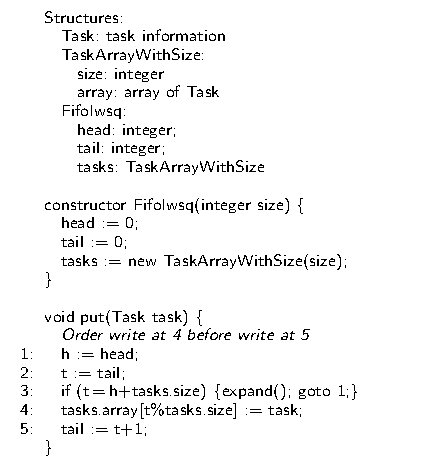
\includegraphics[width=0.5\textwidth, height=0.5\textwidth,keepaspectratio]{contents/figures/IV_6_idempotent-fifo-1.pdf}}
    \subfloat{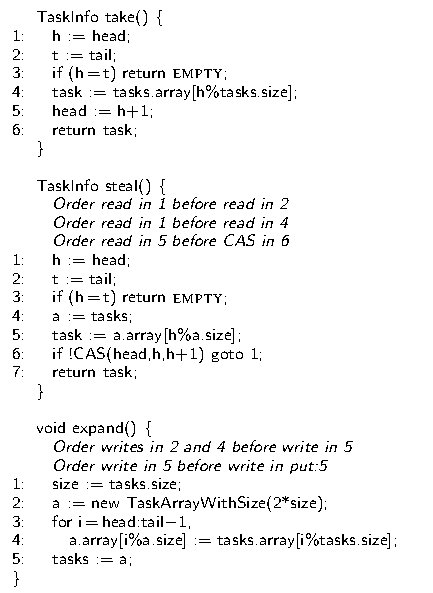
\includegraphics[width=0.5\textwidth, height=0.55\textwidth,keepaspectratio]{contents/figures/IV_6_idempotent-fifo-2.pdf}}
    \caption{\label{fig-idempotent-fifo}Idempotent FIFO work-stealing~\cite{maged.vechev.2009}.}
\end{figure}

Figure~\ref{fig-idempotent-fifo} shows the FIFO idempotent work-stealing algorithm~\cite{maged.vechev.2009}. The algorithm stores the tasks in a shared array $tasks$, and shared integers $head$, and $tail$ indicate the positions of the head and the tail.  For every integer $z > 0$, we describe an execution of the algorithm in which, for every $k \in \{1, \hdots, z\}$, there is a task that is extracted by $\Theta(k)$ distinct operations (possibly by the same thief), with only one of them being concurrent with the others.

\begin{enumerate}

\item Let the owner execute alone $z$ times \Put. Thus, there are $z$ distinct tasks in $tasks$

\item Let $r = z$.

\item The owner executes \Take and stops before executing Line~5, i.e.  it is about to increment $head$.

\item In some order, the thieves sequentially execute $r$ \Steal operations; note these \Steal operations return the $r$ tasks in $tasks[0, \hdots, r-1]$.

\item We now let the owner increment $head$. If $r > 1$, go to step 3 with $r$ decremented by one; else, end the execution.
\end{enumerate}

Observe that in the execution just described, the task in $tasks[i]$, $i \in \{0, \hdots, z-1\}$, is extracted by a \Take operation and by $i+1$ distinct non-concurrent \Steal operations (possible by the same thief).  Thus, the task is extracted $\Theta(i)$ distinct times.  Since $z$ is any positive integer, we conclude there is no bound on the number of times a task can be extracted.

A similar argument works for the other two idempotent work-stealing algorithms.  Ultimately, this happens in all algorithms because tasks are not marked as taken in the shared array where they are stored. Thus, when the owner takes a task and experiences a delay before updating the head/tail, all concurrent modifications of the head/tail performed by the thieves are overwritten once the owner completes its operation, leaving all taken tasks ready to be retaken.  This situation is avoided in our algorithms by marking the entries of the $Tasks$ array as taken and with the help of $\MaxReg$ and $\RangeMaxReg$.


%%% Local Variables:
%%% mode: LaTeX
%%% TeX-master: "../../main"
%%% End:
